\documentclass{article}%
\usepackage[T1]{fontenc}%
\usepackage[utf8]{inputenc}%
\usepackage{lmodern}%
\usepackage{textcomp}%
\usepackage{lastpage}%
\usepackage{geometry}%
\geometry{tmargin=1.5cm,lmargin=1.5cm,rmargin=1.5cm}%
\usepackage{amsmath}%
\usepackage{amsopn}%
\usepackage{breqn}%
\usepackage{pgf}%
\usepackage{pgfplots}%
\usepackage{pdfpages}%
\usepackage{mathtools}%
\usepackage{enumitem}%
\usepackage{xcolor}%
%
\title{Topology Optimization with the Optimality Criteria Method}%
\author{Bence Balogh}%
\date{\today}%
%
\begin{document}%
\normalsize%
\maketitle%
\tableofcontents%
\newpage%
\section{Input}%
\label{sec:Input}%

        \begin{enumerate}
        \item  Lx = 3
        \item  Ly = 3
        \item  E = 12.000
        \item  nu = 0.3
        \end{enumerate}
        %

        \begin{enumerate}[label*=\protect\fbox{MR\arabic{enumi}},
        itemindent=5em]
        \item   normals to the midsurface remain normal
        \item   the plate thickness does not change during deformation
        \item   normal stress through the thickness is ignored
        \end{enumerate}
        

%
\section{Output}%
\label{sec:Output}%

        \begin{figure}[htp] \centering{
        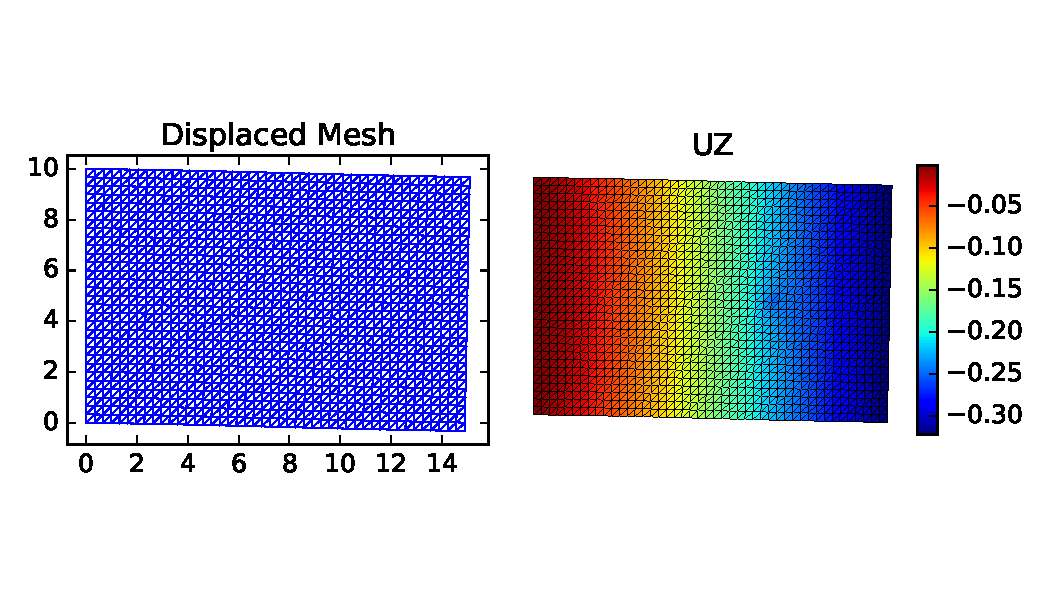
\includegraphics[scale=1.0]{simp_oc_membrane.pdf}}
        \caption{Experiment 1}
        \end{figure}  
        

%
\end{document}